%
% Chapter 6
%

\chapter{DATA AND MC SAMPLES}
This analysis is essentially a counting experiment that compares the number of \tth events predicted with the number of events observed after accounting for the backgrounds.
Simply put, this analysis compares the number of signal + background events predicted by MC to the number of events observed in real data taken by CMS, in the signal regions, after accounting for uncertainties. 
The hypothesis in this case is that the \tth process and all relevant\footnote{Here, relevant means any background capable of entering the signal regions.} backgrounds exist in the amounts dictated by
the Standard Model, and this hypothesis is represented by the MC. 

\section{Data samples}
The data in this analysis was collected from CMS throughout 2016 and only when the magnet was on\footnote{The CMS solenoid was notoriously problematic for datataking during 2015,
suffering from cryogenics issues related to the coldbox and rendering much of the data collected during that time useless from the perspective of most (but not all) physics analyses.}
and all subdetectors were fully operational.
The full 2016 dataset analyzed here corresponds to a total integrated luminosity of 35.9 fb$^{-1}$ and uses the single and double lepton datasets listed in table~\ref{tab:datasets}
and reconstructed with the \texttt{CMSSW\_8\_0\_x} software. This data corresponds to a center-of-mass energy of 13 TeV, and the spacing between bunches in the LHC was 25ns.
On average, there were 30 pileup events per bunch crossing in this data. This data was certified as ``good'' for data analysis internally by CMS~\cite{json}.
The global tags\footnote{The global tag is a CMS-specific parameter that automatically sets all subdetector alignment conditions and calibrations.} used to reconstruct and analyze this data are
\texttt{80X\_dataRun2\_2016SeptRepro\_v7}, corresponding to dataset eras B-G, and \texttt{80X\_dataRun2\_Prompt\_v16} corresponding to era H.

\begin{landscape}
%\setlength\LTcapwidth{5.5in}
%\begin{longtable}{lcp{4.5in}}
\begin{longtable}{p{4.5in}cr}
  \caption[Data samples]{Datasets \label{tab:datasets} }\\
  \toprule
 Dataset & Run Range & Luminosity $\mathrm{fb}^{-1}$ \\

  \midrule
\endfirsthead
  \caption[]{{\em Continued}} \\  % Just like in Chp. 2
  \midrule
 Dataset & Run Range & Luminosity $\mathrm{fb}^{-1}$ \\
  \midrule
\endhead
\endfoot
  \bottomrule
\endlastfoot

\texttt{/SingleElectron/Run2016B-23Sep2016-v3/MINIAOD} & $273150$--$275376$ & $5.79$ \\
\texttt{/SingleElectron/Run2016C-23Sep2016-v1/MINIAOD} & $275656$--$276283$ & $2.57$ \\
\texttt{/SingleElectron/Run2016D-23Sep2016-v1/MINIAOD} & $276315$--$276811$ & $4.25$ \\
\texttt{/SingleElectron/Run2016E-23Sep2016-v1/MINIAOD} & $276831$--$277420$ & $4.01$ \\
\texttt{/SingleElectron/Run2016F-23Sep2016-v1/MINIAOD} & $277932$--$278808$ & $3.10$ \\
\texttt{/SingleElectron/Run2016G-23Sep2016-v1/MINIAOD} & $278820$--$280385$ & $7.54$ \\
\texttt{/SingleElectron/Run2016H-PromptReco-v2/MINIAOD} & $281207$--$284035$ & $8.39$ \\
\texttt{/SingleElectron/Run2016H-PromptReco-v3/MINIAOD} & $284036$--$284044$ & $0.22$ \\
\midrule
\texttt{/SingleMuon/Run2016B-23Sep2016-v3/MINIAOD} & $273150$--$275376$ & $5.79$ \\
\texttt{/SingleMuon/Run2016C-23Sep2016-v1/MINIAOD} & $275656$--$276283$ & $2.57$ \\
\texttt{/SingleMuon/Run2016D-23Sep2016-v1/MINIAOD} & $276315$--$276811$ & $4.25$ \\
\texttt{/SingleMuon/Run2016E-23Sep2016-v1/MINIAOD} & $276831$--$277420$ & $4.01$ \\
\texttt{/SingleMuon/Run2016F-23Sep2016-v1/MINIAOD} & $277932$--$278808$ & $3.10$ \\
\texttt{/SingleMuon/Run2016G-23Sep2016-v1/MINIAOD} & $278820$--$280385$ & $7.54$ \\
\texttt{/SingleMuon/Run2016H-PromptReco-v2/MINIAOD} & $281207$--$284035$ & $8.39$ \\
\texttt{/SingleMuon/Run2016H-PromptReco-v3/MINIAOD} & $284036$--$284044$ & $0.22$ \\
\midrule
\texttt{/DoubleEG/Run2016B-23Sep2016-v3/MINIAOD} & $273150$--$275376$ & $5.79$ \\
\texttt{/DoubleEG/Run2016C-23Sep2016-v1/MINIAOD} & $275656$--$276283$ & $2.57$ \\
\texttt{/DoubleEG/Run2016D-23Sep2016-v1/MINIAOD} & $276315$--$276811$ & $4.25$ \\
\texttt{/DoubleEG/Run2016E-23Sep2016-v1/MINIAOD} & $276831$--$277420$ & $4.01$ \\
\texttt{/DoubleEG/Run2016F-23Sep2016-v1/MINIAOD} & $277932$--$278808$ & $3.10$ \\
\texttt{/DoubleEG/Run2016G-23Sep2016-v1/MINIAOD} & $278820$--$280385$ & $7.54$ \\
\texttt{/DoubleEG/Run2016H-PromptReco-v2/MINIAOD} & $281207$--$284035$ & $8.39$ \\
\texttt{/DoubleEG/Run2016H-PromptReco-v3/MINIAOD} & $284036$--$284044$ & $0.22$ \\
\midrule
\texttt{/DoubleMuon/Run2016B-23Sep2016-v3/MINIAOD} & $273150$--$275376$ & $5.79$ \\
\texttt{/DoubleMuon/Run2016C-23Sep2016-v1/MINIAOD} & $275656$--$276283$ & $2.57$ \\
\texttt{/DoubleMuon/Run2016D-23Sep2016-v1/MINIAOD} & $276315$--$276811$ & $4.25$ \\
\texttt{/DoubleMuon/Run2016E-23Sep2016-v1/MINIAOD} & $276831$--$277420$ & $4.01$ \\
\texttt{/DoubleMuon/Run2016F-23Sep2016-v1/MINIAOD} & $277932$--$278808$ & $3.10$ \\
\texttt{/DoubleMuon/Run2016G-23Sep2016-v1/MINIAOD} & $278820$--$280385$ & $7.54$ \\
\texttt{/DoubleMuon/Run2016H-PromptReco-v2/MINIAOD} & $281207$--$284035$ & $8.39$ \\
\texttt{/DoubleMuon/Run2016H-PromptReco-v3/MINIAOD} & $284036$--$284044$ & $0.22$ \\
\midrule
\texttt{/MuonEG/Run2016B-23Sep2016-v3/MINIAOD} & $273150$--$275376$ & $5.79$ \\
\texttt{/MuonEG/Run2016C-23Sep2016-v1/MINIAOD} & $275656$--$276283$ & $2.57$ \\
\texttt{/MuonEG/Run2016D-23Sep2016-v1/MINIAOD} & $276315$--$276811$ & $4.25$ \\
\texttt{/MuonEG/Run2016E-23Sep2016-v1/MINIAOD} & $276831$--$277420$ & $4.01$ \\
\texttt{/MuonEG/Run2016F-23Sep2016-v1/MINIAOD} & $277932$--$278808$ & $3.10$ \\
\texttt{/MuonEG/Run2016G-23Sep2016-v1/MINIAOD} & $278820$--$280385$ & $7.54$ \\
\texttt{/MuonEG/Run2016H-PromptReco-v2/MINIAOD} & $281207$--$284035$ & $8.39$ \\
\texttt{/MuonEG/Run2016H-PromptReco-v3/MINIAOD} & $284036$--$284044$ & $0.22$ \\

\end{longtable}
\end{landscape}

\section{MC samples}
The collection of MC samples described below comprise both the signal and background predictions. 
Like the data, the software used for MC simulation was \texttt{CMSSW\_8\_0\_x}.


%%notes about how MC is generated
While several different generators were used to produce the MC in this analysis, the basic strategy is the same.
A given generator uses next-to-leading-order (NLO)\footnote{While the signal and dominant background MC is produced
at NLO, some smaller backgrounds are generated only to leading-order precision.}
matrix element calculations to generate events based on hard scatter
interactions between the initial state partons. These initial state partons are simulating the
actual proton collison inside CMS. The initial partons used in the MC generation are sampled from the parton
distribution functions (PDFs) which dictate the abundance of each parton flavor for the proton at a given momentum transfer.
Then the matrix element calculation is performed resulting in the final state particles. At this point, the shower simulation
begins by taking the final state particles from the matrix element and simulating their decay/hadronization. Since this step
cannot be calculated with perturbative QCD, it is instead handled by fragmentation functions which attempt to mimic a real
hadronization as accuartely as possible. At this stage, the event generation portion of the MC production (called the ``GEN'' step)
is complete and the interaction with the dector must be simulated. This simulation is carried out with the GEANT4 software package,
which models the CMS detector, as well as the GEN particles hits, tracks, energy deposits and other interactions that occur
between the particles produced from the GEN step and the CMS detector simulation (called the ``SIM'' step). Next, the simulated
hits are converted into a digitized detector response, which is designed to recreate the response of the actual detector as
closely as possible. This stage, called the ``DIGI'' step, also includes the emulated trigger accept/reject decisions and is the
first place where MC is directly comparable to data. The final step\footnote{Technically there is an additional step where RECO data
is converted into Analysis Object Data (AOD). This includes a slimming of attributes wrt RECO, and reconstructing high-level objects
used in the analysis.} called ``RECO'', is the reconstruction of high-level objects such as jets, tracks, and MET from hits and
energy deposits. This RECO step is functionally identical between the real data collected by CMS and the MC simulation, allowing
for a direct comparison between MC and real data at the RECO tier, and where the physics analysis begins. An overview of the entire
data chain from initial interaction to analysis objects is in Figure~\ref{fig:data_mc_chain}.

\begin{figure}[hbtp]
 \begin{center}
   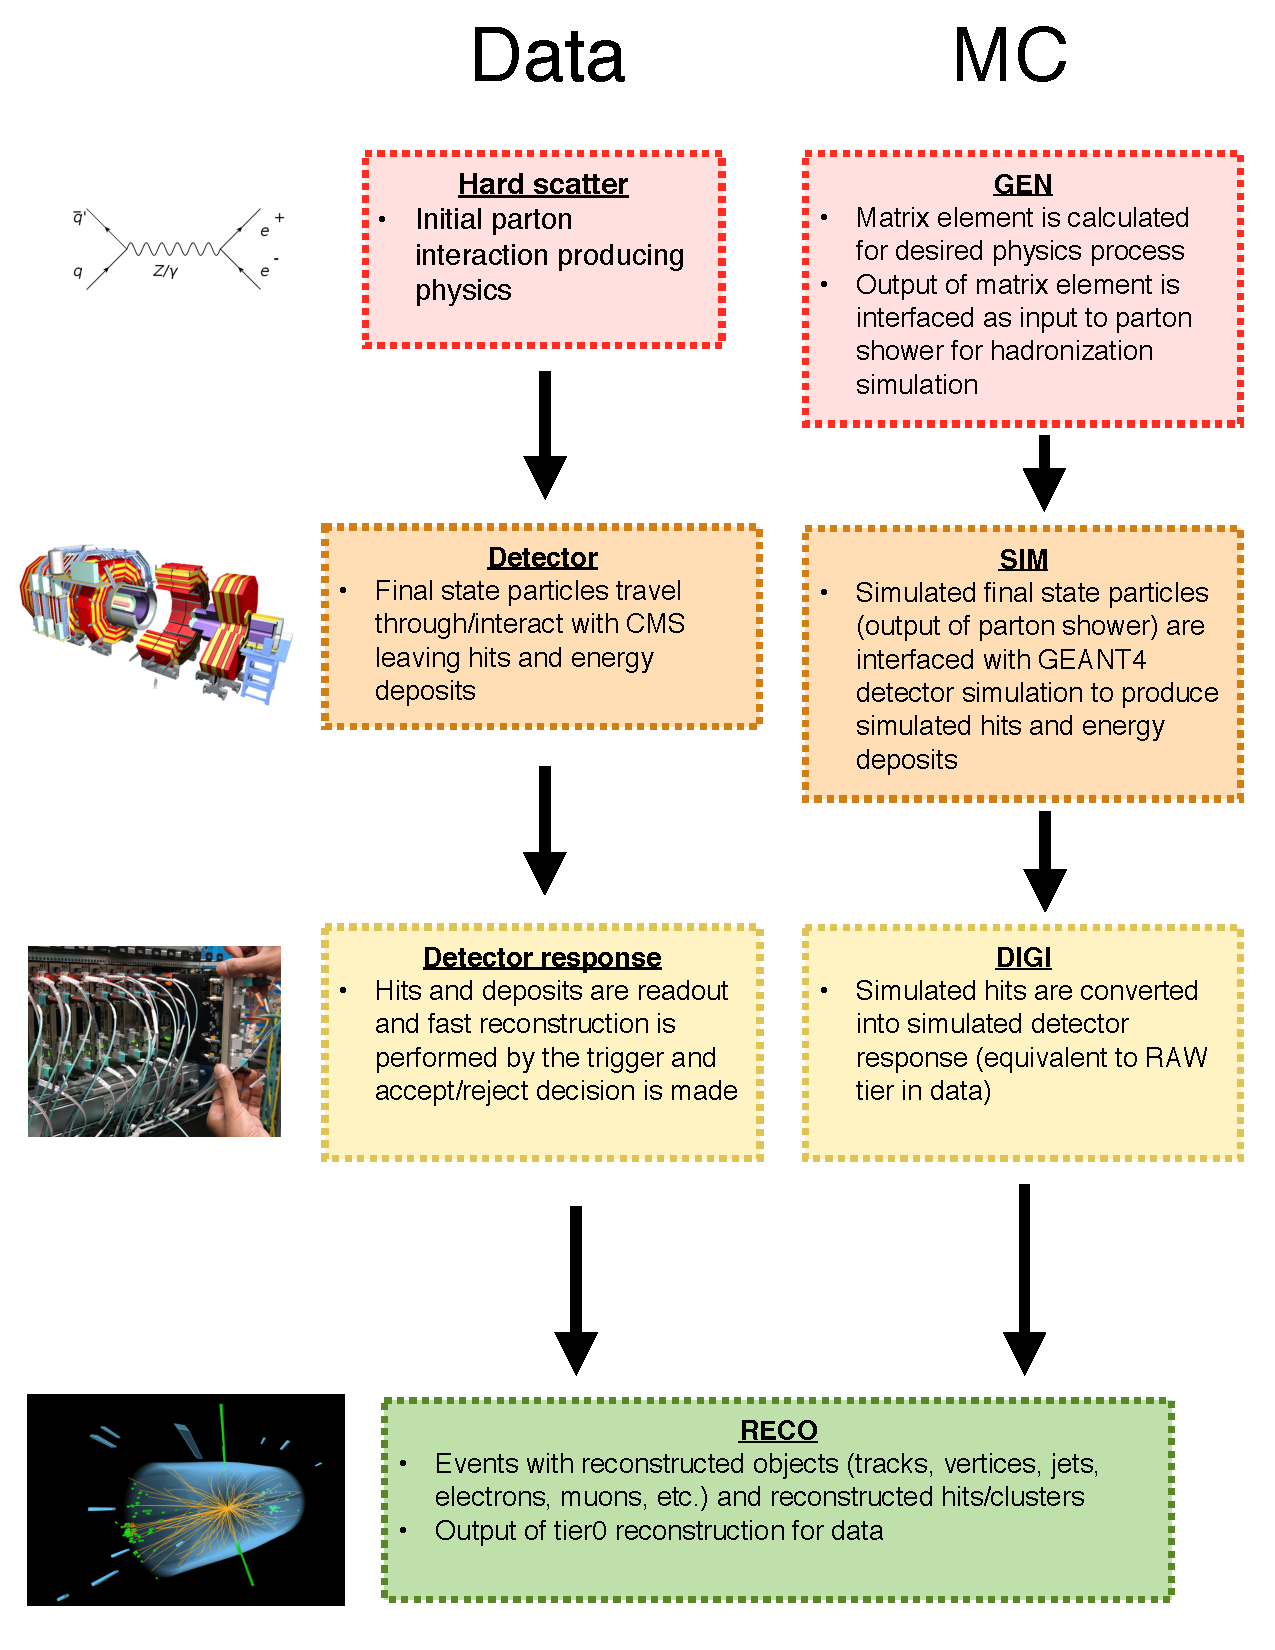
\includegraphics[width=0.9\textwidth]{ch6_figs/data_mc_diagram.pdf}
   \caption[Diagram comparing data taking and MC generation stages]{An overview and comparison of the data taking and MC generation stages.~\cite{cms_pflow_img}.}
   \label{fig:data_mc_chain}
 \end{center}
\end{figure}

\subsection{Signal}
The signal MC sample is produced with the \textsc{POWHEG} generator at NLO~\cite{powheg}, assuming a Higgs boson mass of 125 GeV and using the \textsc{NNPDF3.0} for the proton
PDFs~\cite{nnpdf3}. The shower process is simulated by \textsc{PYTHIA}~\cite{pythia} with the \textsc{CUETP8M2T4} tune to improve the modeling of the multiplicity~\cite{CUETP8M2T4}. 
The signal sample considers all decays of the Higgs boson except those to quarks and the cross section is modified accordingly, this is useful because no resources are wasted filtering
and storing events that would not pass the signal regions. 

\subsection{Backgrounds}
The majority\footnote{The backgrounds estimated via data-driven methods are described in detail later.} of the background predictions in this analysis are MC-based estimations. 
The leading MC background estimations are generated with \textsc{MadGraph5$\_$aMC$\@$NLO} with shower simulated by \textsc{POWHEG}~\cite{aMCatNLO,nlo_showerMC,powheg}. The remaining 
backgrounds generated and showered with one of the generators and shower MC already mentioned.   

\begin{landscape}
%%\setlength\LTcapwidth{6.5in}
%\begin{longtable}{lcp{4.5in}}
%\begin{longtable}{p{4.5in}cr}
%\begin{longtable}{lp{4.5in}c}
\begin{longtable}{lp{6.0in}r}
  \caption[MC Samples]{Monte-Carlo samples used in this analysis. The first section is the sample used for signal prediction, the second section contains the largest backgrounds
that are predicted by MC, the third section contains the samples for other, non-dominant SM backgrounds, the fourth section lists the rare SM backgrounds, and the final section
contains the samples used in control regions, that don't directly enter the final yields or discriminant shapes.\label{tab:mc} }\\
  \toprule
 Process & MC sample & Cross-section [pb] \\

  \midrule
\endfirsthead
  \caption[]{{\em Continued}} \\  % Just like in Chp. 2
  \midrule
 Process & MC sample & Cross-Section [pb] \\
  \midrule
\endhead
\endfoot
  \bottomrule
\endlastfoot

\tth & \texttt{/ttHJetToNonbb\_M125\_13TeV\_amcatnloFXFX\_madspin\_pythia8\_mWCutfix/}$^{3}$ & $2.15 \times 10^{-1}$ \\
\midrule
\ttw & \texttt{/TTWJetsToLNu\_TuneCUETP8M1\_13TeV-amcatnloFXFX-madspin-pythia8/}$^{2,5}$ & $2.04 \times 10^{-1}$ \\
\ttz & \texttt{/TTZToLLNuNu\_M-10\_TuneCUETP8M1\_13TeV-amcatnlo-pythia8/}$^{3}$ & $2.73 \times 10^{-1}$ \\
\midrule
$t\bar{t}+\gamma+$jets & \texttt{/TTGJets\_TuneCUETP8M1\_13TeV-amcatnloFXFX-madspin-pythia8/}$^{1}$ & $3.70$ \\
$t+\gamma+$jets & \texttt{/TGJets\_TuneCUETP8M1\_13TeV\_amcatnlo\_madspin\_pythia8/}$^{1}$ & $2.97$ \\
$W+\gamma+$jets & \texttt{/WGToLNuG\_TuneCUETP8M1\_13TeV-amcatnloFXFX-pythia8/}$^{3}$ & $5.86 \times 10^{2}$ \\
$Z/\gamma+$jets & \texttt{/ZGTo2LG\_TuneCUETP8M1\_13TeV-amcatnloFXFX-pythia8/}$^{3}$ & $1.31 \times 10^{2}$ \\
$WW$ & \texttt{/WWTo2L2Nu\_13TeV-powheg/}$^{1}$ & $1.05 \times 10^{1}$ \\
$WW$ & \texttt{/WWTo2L2Nu\_DoubleScattering\_13TeV-pythia8/}$^{1}$ & $1.73 \times 10^{-1}$ \\
$WW$ & \texttt{/WpWpJJ\_13TeV-powheg-pythia8/}$^{2}$ & $3.71 \times 10^{-2}$ \\
\midrule
$WZ$ & \texttt{/WZTo3LNu\_TuneCUETP8M1\_13TeV-powheg-pythia8}$^{1}$ & $4.43$ \\
$ZZ$ & \texttt{/ZZTo4L\_13TeV-amcatnloFXFX-pythia8/}$^{3}$ & $1.26$ \\
$WWW$ & \texttt{/WWW\_4F\_TuneCUETP8M1\_13TeV-amcatnlo-pythia8/}$^{1}$ & $2.09 \times 10^{-1}$ \\
$WWZ$ & \texttt{/WWZ\_TuneCUETP8M1\_13TeV-amcatnlo-pythia8/}$^{1}$ & $1.65 \times 10^{-1}$ \\
$WZZ$ & \texttt{/WZZ\_TuneCUETP8M1\_13TeV-amcatnlo-pythia8/}$^{1}$ & $5.57 \times 10^{-2}$ \\
$ZZZ$ & \texttt{/ZZZ\_TuneCUETP8M1\_13TeV-amcatnlo-pythia8/}$^{1}$ & $1.40 \times 10^{-2}$ \\
$t+Z$ & \texttt{/tZq\_ll\_4f\_13TeV-amcatnlo-pythia8/}$^{3}$ & $7.58 \times 10^{-2}$ \\
$tt\bar{t}\bar{t}$ & \texttt{/TTTT\_TuneCUETP8M2T4\_13TeV-amcatnlo-pythia8/}$^{1}$ & $9.10 \times 10^{-3}$ \\
\midrule
$t\bar{t}+$jets & \texttt{/TTJets\_DiLept\_TuneCUETP8M1\_13TeV-madgraphMLM-pythia8/}$^{1,3}$ & $8.73 \times 10^{1}$ \\
$t\bar{t}+$jets & \texttt{/TTJets\_SingleLeptFromT\_TuneCUETP8M1\_13TeV-madgraphMLM-pythia8/}$^{1}$ & $1.82 \times 10^{1,2}$ \\
$t\bar{t}+$jets & \texttt{/TTJets\_SingleLeptFromTbar\_TuneCUETP8M1\_13TeV-madgraphMLM-pythia8/}$^{3}$ & $1.82 \times 10^{1,2}$ \\
$Z/\gamma^{*}\rightarrow ll$ & \texttt{/DYJetsToLL\_M-10to50\_TuneCUETP8M1\_13TeV-amcatnloFXFX-pythia8/}$^{1}$ & $6.03 \times 10^{3}$ \\
$Z/\gamma^{*}\rightarrow ll$ & \texttt{/DYJetsToLL\_M-50\_TuneCUETP8M1\_13TeV-madgraphMLM-pythia8/}$^{4}$ & $5.77 \times 10^{3}$ \\
$W+$jets & \texttt{/WJetsToLNu\_TuneCUETP8M1\_13TeV-amcatnloFXFX-pythia8/}$^{1}$ & $6.15 \times 10^{4}$ \\
$t$ & \texttt{/ST\_s-channel\_4f\_leptonDecays\_13TeV-amcatnlo-pythia8\_TuneCUETP8M1/}$^{1}$ & $3.68$ \\
$t$ & \texttt{/ST\_t-channel\_top\_4f\_inclusiveDecays\_13TeV-powhegV2-madspin-pythia8\_TuneCUETP8M1/}$^{1}$ & $1.36 \times 10^{2}$ \\
$\bar{t}$ & \texttt{/ST\_t-channel\_antitop\_4f\_inclusiveDecays\_13TeV-powhegV2-madspin-pythia8\_TuneCUETP8M1/}$^{1}$ & $8.10 \times 10^{1}$ \\
$tW$ & \texttt{/ST\_tW\_top\_5f\_inclusiveDecays\_13TeV-powheg-pythia8\_TuneCUETP8M1/}$^{3}$ & $3.56 \times 10^{1}$ \\
$\bar{t}W$ & \texttt{/ST\_tW\_antitop\_5f\_inclusiveDecays\_13TeV-powheg-pythia8\_TuneCUETP8M1/}$^{3}$ & $3.56 \times 10^{1}$ \\

\end{longtable}
{\footnotesize
$^{1}$ \texttt{RunIISummer16MiniAODv2-PUMoriond17\_80X\_mcRun2\_asymptotic\_2016\_TrancheIV\_v6-v1/MINIAODSIM} \\
$^{2}$ \texttt{RunIISummer16MiniAODv2-PUMoriond17\_80X\_mcRun2\_asymptotic\_2016\_TrancheIV\_v6\_ext2-v1/MINIAODSIM} \\
$^{3}$ \texttt{RunIISummer16MiniAODv2-PUMoriond17\_80X\_mcRun2\_asymptotic\_2016\_TrancheIV\_v6\_ext1-v1/MINIAODSIM} \\
$^{4}$ \texttt{RunIISummer16MiniAODv2-PUMoriond17\_80X\_mcRun2\_asymptotic\_2016\_TrancheIV\_v6\_ext1-v2/MINIAODSIM} \\
$^{5}$ \texttt{RunIISummer16MiniAODv2-PUMoriond17\_80X\_mcRun2\_asymptotic\_2016\_TrancheIV\_v6\_ext1-v3/MINIAODSIM} \\
} % end footnotesize

\end{landscape}


\section{Triggers}
The triggers used in this analysis are choosen to select events with one or more leptons, which are the events with the greatest
chance of passing the signal region selection. We consider triggers that fire on events with one, two, or three leptons. The primary
requirement and defining characteristic of the lepton triggers is the pt of the lepton.
Although all signal regions require at least two leptons, considering events where only a single-lepton trigger fired boosts acceptance, since
we consider events with two or more leptons, but where the sub-leading (in terms of \pt) lepton failed to pass the requirements of the
double or triple lepton trigger. To further boost event acceptance, we use the logical 'OR' of all trigger decisions in each signal
region category described in Table~\ref{tab:triggers}. While additional single, double, and triple lepton triggers are available,
in the CMS HLT menu, we use \emph{only} the lowest-threshold, unprescaled\footnote{Because the HLT, DAQ and downstream hardware can only handle a maximum trigger
rate, the trigger menu
uses prescales to control the rates of trigger that would otherwise fire too often. This allows lower-priority triggers to collect data
without consuming large rates. The prescale control how frequency a trigger fires. For example a trigger with a prescale of 2 means that
data is recorded every other time the trigger fires.} triggers to maximize efficiency and to make the luminosity calculation and trigger efficiency measurements
straightforward and simple. 

\begin{longtable}{l}
\caption[Trigger list]{Triggers used in this analysis.\label{tab:triggers}}\\
\hline
$2lss~(\mu\mu)$ \\
\hline
HLT$\_$Mu17$\_$TrkIsoVVL$\_$Mu8$\_$TrkIsoVVL$\_$DZ$\_$v* \\
HLT$\_$Mu17$\_$TrkIsoVVL$\_$TkMu8$\_$TrkIsoVVL$\_$DZ$\_$v* \\
HLT$\_$IsoMu22$\_$v* \\
HLT$\_$IsoTkMu22$\_$v* \\
HLT$\_$IsoMu22$\_$eta2p1$\_$v* \\
HLT$\_$IsoTkMu22$\_$eta2p1$\_$v* \\
HLT$\_$IsoMu24$\_$v* \\
HLT$\_$IsoTkMu24$\_$v* \\
\hline
\hline
$2lss~(ee)$ \\
\hline
HLT$\_$Ele23$\_$Ele12$\_$CaloIdL$\_$TrackIdL$\_$IsoVL$\_$DZ$\_$v* \\
HLT$\_$Ele27$\_$WPTight$\_$Gsf$\_$v* \\
HLT$\_$Ele25$\_$eta2p1$\_$WPTight$\_$Gsf$\_$v* \\
HLT$\_$Ele27$\_$eta2p1$\_$WPLoose$\_$Gsf$\_$v* \\
\hline
\hline
$2lss~(e\mu)$ \\
\hline
HLT$\_$Mu23$\_$TrkIsoVVL$\_$Ele8$\_$CaloIdL$\_$TrackIdL$\_$IsoVL$\_$v* \\
HLT$\_$Mu23$\_$TrkIsoVVL$\_$Ele8$\_$CaloIdL$\_$TrackIdL$\_$IsoVL$\_$DZ$\_$v* \\
HLT$\_$Mu8$\_$TrkIsoVVL$\_$Ele23$\_$CaloIdL$\_$TrackIdL$\_$IsoVL$\_$v* \\
HLT$\_$Mu8$\_$TrkIsoVVL$\_$Ele23$\_$CaloIdL$\_$TrackIdL$\_$IsoVL$\_$DZ$\_$v* \\
HLT$\_$IsoMu22$\_$v* \\
HLT$\_$IsoTkMu22$\_$v* \\
HLT$\_$IsoMu22$\_$eta2p1$\_$v* \\
HLT$\_$IsoTkMu22$\_$eta2p1$\_$v* \\
HLT$\_$IsoMu24$\_$v* \\
HLT$\_$IsoTkMu24$\_$v* \\
HLT$\_$Ele23$\_$Ele12$\_$CaloIdL$\_$TrackIdL$\_$IsoVL$\_$DZ$\_$v* \\
HLT$\_$Ele27$\_$WPTight$\_$Gsf$\_$v* \\
HLT$\_$Ele25$\_$eta2p1$\_$WPTight$\_$Gsf$\_$v* \\
HLT$\_$Ele27$\_$eta2p1$\_$WPLoose$\_$Gsf$\_$v* \\
\hline
\end{longtable}

%%%discuss used triggers
The trigger efficiency is measured separately in data and MC. Measuring the trigger efficiency accurately and precisely is critically
important in a sensitive physics analysis. This is because the trigger effiency directly scales the luminosity, and thus the number
of events in the counting experiment.
Because this efficiency differs slightly between data and MC, we correct the MC efficiency with scale factors to match the
efficiency in data. The trigger efficiency measured in data is performed by selecting data that was recorded on triggers completely
uncorrelated with the lepton triggers used in this analysis. The data used for the efficiency measurement is recorded by triggers in
the MET dataset so there is no implicit bias in the sample, because the triggers that collected the data are different from the triggers
for which we are measuring the efficiency. With the MET dataset, we select events with two and three loose leptons separately, we then measure
the efficiency for the candidate events to pass the 'OR' of all triggers in the respective category. This effiency can then be compared
to that measured in the MC, and we obtain the scale factors listed in Table~\ref{tab:trigger_sf}. We observe an excellent agreement between
the efficiencies measured in data to that in MC. 

%discuss trigger scale factors 

\begin{table}[hbtp]
\centering
\caption{Trigger efficiency scale factors and uncertainties.}
\begin{tabular}{l|l}
\hline
Category & Scale Factor \\
\hline
$2lss (ee)$ & 1.01$\pm$0.02 \\
$2lss (e\mu)$ & 1.01$\pm$0.01 \\
$2lss (\mu\mu)$ & 1.00$\pm$0.01 \\
\hline
\end{tabular}
\label{tab:trigger_sf}
\end{table}

The triggers are the first place where the object selection is introduced into the analysis, and while the efficiency is high and closes well,
the object selection defined in the analysis must be strictly tighter than the object selection definied in any of the triggers. This ensures
the efficiency is well-measured and does not vary with the lepton \pt or $|\eta|$, that is the effiency is taken past the ``turn-on'' curve
of efficiency in Figures~\ref{fig:trigeffsmumu,fig:trigeffsemu,fig:trigeffsee}  

\begin{figure}[htp]
\centering
\includegraphics[width=0.49\textwidth]{ch6_figs/1D_eff_lep1_pt_uu_ARCv2_change_3l_pt_ranges.pdf}
\includegraphics[width=0.49\textwidth]{ch6_figs/1D_eff_lep2_pt_uu_ARCv2_change_3l_pt_ranges.pdf} \\
\includegraphics[width=0.49\textwidth]{ch6_figs/1D_eff_lep1_eta_uu_ARCv2_change_3l_pt_ranges.pdf}
\includegraphics[width=0.49\textwidth]{ch6_figs/1D_eff_lep2_eta_uu_ARCv2_change_3l_pt_ranges.pdf}
\caption[Trigger efficiency in the 2lss $\mu\mu$ category]{Comparison of the trigger efficiency in the same-sign dimuon category before 
corrections, shown as a function of the \pt and $\eta$ of the leading lepton (left) 
and the sub-leading lepton (right).}
\label{fig:trigeffsmumu}
\end{figure}

\begin{figure}[htp]
\centering
\includegraphics[width=0.49\textwidth]{ch6_figs/1D_eff_lep1_pt_eu_ARCv2_change_3l_pt_ranges.pdf}
\includegraphics[width=0.49\textwidth]{ch6_figs/1D_eff_lep2_pt_eu_ARCv2_change_3l_pt_ranges.pdf} \\
\includegraphics[width=0.49\textwidth]{ch6_figs/1D_eff_lep1_eta_eu_ARCv2_change_3l_pt_ranges.pdf}
\includegraphics[width=0.49\textwidth]{ch6_figs/1D_eff_lep2_eta_eu_ARCv2_change_3l_pt_ranges.pdf}
\caption[Trigger efficiency in the 2lss $e\mu$ category]{Comparison of the trigger efficiency in the same-sign muon+electron category before 
corrections, shown as a function of the \pt and $\eta$ of the leading lepton (left) 
and the sub-leading lepton (right).}
\label{fig:trigeffsemu}
\end{figure}

\begin{figure}[htp]
\centering
\includegraphics[width=0.49\textwidth]{ch6_figs/1D_eff_lep1_pt_ee_ARCv2_change_3l_pt_ranges.pdf}
\includegraphics[width=0.49\textwidth]{ch6_figs/1D_eff_lep2_pt_ee_ARCv2_change_3l_pt_ranges.pdf} \\
\includegraphics[width=0.49\textwidth]{ch6_figs/1D_eff_lep1_eta_ee_ARCv2_change_3l_pt_ranges.pdf}
\includegraphics[width=0.49\textwidth]{ch6_figs/1D_eff_lep2_eta_ee_ARCv2_change_3l_pt_ranges.pdf}
\caption[Trigger efficiency in the 2lss $ee$ category]{Comparison of the trigger efficiency in the same-sign dielectron category before 
corrections, shown as a function of the \pt and $\eta$ of the leading lepton (left) 
and the sub-leading lepton (right).}
\label{fig:trigeffsee}
\end{figure}



%% \begin{figure}[hbtp]
%%  \begin{center}
%%    \includegraphics[width=0.8\textwidth]{ch4_figs/cms_particleflow.pdf}
%%    \caption{An overview of how CMS detects different types of particles. The slice of CMS in in the x-y plane.~\cite{NEED CITATION}.}
%%    \label{fig:cms_pflow}
%%  \end{center}
%% \end{figure}
